%%%%%%%%%%%%%%%%%%%%%%%%%%%%%%%%%%%%%%%%%%%%%%%%%%%%%%%%%%%%%%%%%%%%%%%%%%%%%%%%
%%%%%%%%%%%%%%%%%%%%%%%%%%%%%%%%%%%%%%%%%%%%%%%%%%%%%%%%%%%%%%%%%%%%%%%%%%%%%%%%
%
% A general frame for lecture slides and lecture notes in one file
% using LaTeX beamer
%
%%%%%%%%%%%%%%%%%%%%%%%%%%%%%%%%%%%%%%%%%%%%%%%%%%%%%%%%%%%%%%%%%%%%%%%%%%%%%%%%
%%%%%%%%%%%%%%%%%%%%%%%%%%%%%%%%%%%%%%%%%%%%%%%%%%%%%%%%%%%%%%%%%%%%%%%%%%%%%%%%
\documentclass[ignorenonframetext,11pt]{beamer}
%\usepackage[ngerman]{babel}
%\usepackage[T1]{fontenc}
\usepackage[utf8]{inputenc}
\usepackage{lmodern}
\usepackage{amsmath,amssymb,amsfonts}


% only presentation
\mode<presentation>
{
  \usetheme{default}
%  \usecolortheme{crane}
  \setbeamercovered{transparent}
%  \setlength{\parindent}{0pt}
%  \setlength{\parskip}{1.35ex plus 0.5ex minus 0.3ex}
%  \usefonttheme{structuresmallcapsserif}
  \usefonttheme{structurebold}
  \setbeamertemplate{theorems}[numbered]
  \usepackage{amscd}
}

% all after
\usepackage{tikz}
\usepackage{pgfplots,adjustbox}
\usepackage{eurosym}
\usepackage{graphicx}
\usepackage{multimedia}
\usepackage{psfrag}

\usepackage{listings}
\definecolor{listingbg}{gray}{0.90}
\lstset{language=C++, basicstyle=\ttfamily,
  keywordstyle=\color{black}\bfseries, tabsize=4, stringstyle=\ttfamily,
  commentstyle=\it, extendedchars=true, escapeinside={/*@}{@*/}}

\usepackage{minted}
\usepackage{curves}
%\usepackage{epic}
\usepackage{calc}
%\usepackage{picinpar}
%\usepackage{fancybox}
%\usepackage{xspace}
\usepackage{enumerate}
\usepackage{algpseudocode}
\usepackage{color}
\usepackage{bold-extra}
\usepackage{bm}
\usepackage{stmaryrd}
%\usepackage[squaren]{SIunits}
\usepackage{nicefrac}

\usepackage{fancyvrb,bbm,xspace}
\usepackage{lmodern}
\usepackage{fancyvrb,bbm,xspace}
\usepackage[binary-units]{siunitx}
\usepackage{xcolor,tabu}
\usepackage{booktabs}

\definecolor{niceblue}{rgb}{0.122,0.396,0.651}   %% 31, 101, 166 or #1F65A6
\definecolor{niceorange}{RGB}{255,205,86}        %% #FFCD56
\definecolor{nicered}{RGB}{220,20,60}                      %% rgb(220, 20, 60)
\definecolor{niceteal}{HTML}{00A9AB}
\definecolor{niceviolet}{HTML}{820080}

\definecolor{niceblueLight}{HTML}{91CAFB}
\definecolor{niceblueVeryLight}{HTML}{DDEFFF}

\usepackage{dsfont}

%\newcommand{\hlineabove}{\rule{0pt}{2.6ex}}
%\newcommand{\hlinebelow}{\rule[-1.2ex]{0pt}{0pt}}

%\usecolortheme[RGB={37,75,123}]{structure}
% \definecolor{structurecolor}{rgb}{0.905,0.318,0.071}

% \setbeamercolor{frametitle}{fg=black,bg=}
% \setbeamercolor{sidebar left}{fg=,bg=}

% \setbeamertemplate{headline}{\vskip4em}
% \setbeamersize{sidebar width left=.9cm}

% \setbeamertemplate{navigation symbols}{}
%\setbeamertemplate{blocks}[rounded][shadow=true]
%\setbeamertemplate{itemize items}[square]

\mode<presentation>
{
\theoremstyle{definition}
}
\newtheorem{Def}{Definition}%[section]
\newtheorem{Exm}[Def]{Example}
\newtheorem{Lem}[Def]{Lemma}
\newtheorem{Rem}[Def]{Remark}
\newtheorem{Rul}[Def]{Rule}
\newtheorem{Thm}[Def]{Theorem}
\newtheorem{Cor}[Def]{Corollary}
\newtheorem{Obs}[Def]{Observation}
\newtheorem{Ass}[Def]{Assumption}
\newtheorem{Pro}[Def]{Property}
\newtheorem{Alg}[Def]{Algorithm}
\newtheorem{Prp}[Def]{Proposition}
\newtheorem{Lst}[Def]{Listing}


%% Typesetting C++
\def\CC{{C\nolinebreak[4]\hspace{-.05em}\raisebox{.4ex}{\tiny\bf ++}}}

% Delete this, if you do not want the table of contents to pop up at
% the beginning of each subsection:
\AtBeginSection[]
{
  \begin{frame}<beamer>
    \frametitle{Contents}
    \tableofcontents[sectionstyle=show/shaded,subsectionstyle=hide/hide/hide]
%\tableofcontents[currentsection]
  \end{frame}
}

% Title definition
\mode<presentation>
{
  \title{DUNE PDELab Tutorial 09\\
  {\small  Using code generation to create local operators}}
  \author{PDELab Team}
  \institute[]
  {
   Interdisziplinäres Zentrum für Wissenschaftliches Rechnen\\
   Im Neuenheimer Feld 205, D-69120 Heidelberg \\[6pt]
  }
  \date[\today]{\today}
}


% logo nach oben
\mode<presentation>
{
% No navigation symbols and no lower logo
\setbeamertemplate{sidebar right}{}

% logo
\newsavebox{\logobox}
\sbox{\logobox}{%
    \hskip\paperwidth%
    \rlap{%
      % putting the logo should not change the vertical possition
      \vbox to 0pt{%
        \vskip-\paperheight%
        \vskip0.35cm%
        \llap{\insertlogo\hskip0.1cm}%
        % avoid overfull \vbox messages
        \vss%
      }%
    }%
}

\addtobeamertemplate{footline}{}{%
    \usebox{\logobox}%
}
}

%%%%%%%%%%%%%%%%%%%%%%%%%%%%%%%%%%%%%%%%%%%%%%%%%%%%%%%%%%%%%%%%%%%%%%%%%%%%%%%%
%%%%%%%%%%%%%%%%%%%%%%%%%%%%%%%%%%%%%%%%%%%%%%%%%%%%%%%%%%%%%%%%%%%%%%%%%%%%%%%%
%
% now comes the individual stuff lecture by lecture
%
%%%%%%%%%%%%%%%%%%%%%%%%%%%%%%%%%%%%%%%%%%%%%%%%%%%%%%%%%%%%%%%%%%%%%%%%%%%%%%%%
%%%%%%%%%%%%%%%%%%%%%%%%%%%%%%%%%%%%%%%%%%%%%%%%%%%%%%%%%%%%%%%%%%%%%%%%%%%%%%%%

\begin{document}

\frame{\titlepage}

%%%%%%%%%%%%%%%%%%%%%%%%%%%%%%%%%%%%%%%%%%%%%%%%%%%%%%%%%%%%%%%%%%%%%%%%%%%%%%%%
%%%%%%%%%%%%%%%%%%%%%%%%%%%%%%%%%%%%%%%%%%%%%%%%%%%%%%%%%%%%%%%%%%%%%%%%%%%%%%%%
\section{Introduction}

\begin{frame}[fragile]
  \frametitle{Introduction}
  \textbf{Introduction}
  \begin{itemize}
  \item This tutorial gives a short introduction to using
    \lstinline{dune-codegen}\footnote{https://gitlab.dune-project.org/extensions/dune-codegen}
  \item Partially based on ``Code Generation for High Performance PDE Solvers
    on Modern Architectures'' by Dominic Kempf
  \item Partially based on \url{https://fenics.readthedocs.io/projects/ufl/en/latest/index.html}
  \end{itemize}

  \vfill

  \textbf{Goal}
  \begin{itemize}
  \item Describe weak formulation using a domain-specific language
  \item We use UFL\footnote{https://bitbucket.org/fenics-project/ufl} for this
  \item Generate \CC\ code for the local integration kernels as a PDELab
    \lstinline{LocalOperator}
  \item Make it easier to use PDELab for your application
  \end{itemize}
\end{frame}

\begin{frame}
  \frametitle{Introduction}
  We will look at a quick example to get some idea how this looks like.
\end{frame}

\begin{frame}
  \frametitle{Hello World: Poisson Problem}

  \begin{itemize}
  \item Strong formulation:
    \begin{align*}
      -\Delta u & = f \qquad\text{in $\Omega$}, \\
      u &= g \qquad\text{on $\partial\Omega$},
    \end{align*}
  \item Discrete weak formulation: Find $u_h \in U_h$ with
    \begin{equation*}
      r_h^{Poisson}(u_h, v_h) = \int_\Omega \nabla u_h \cdot \nabla v_h \, dx
      - \int_\Omega f \, v_h \, dx = 0 \qquad \forall v_h \in V_h
    \end{equation*}
  \item Parameter functions:
    \begin{align*}
      f(x) = -2d \\
      g(x) = \| x \|_2^2
    \end{align*}
  \end{itemize}
\end{frame}

\begin{frame}
  \frametitle{UFL file for Poisson Problem}
  % \inputminted[fontsize=\scriptsize]{python}{../src/poisson.ufl}
  \lstinputlisting[basicstyle=\scriptsize, backgroundcolor=\color{listingbg}]{../src/poisson.ufl}
\end{frame}

\begin{frame}
  \frametitle{Goals of this Talk}

  \textbf{Goals of this talk}
  \begin{itemize}
  \item Explain how to write down PDEs in UFL
  \item Show how we modify/extend UFL
  \item Show how it is integrated into the build system
  \end{itemize}
  \vfill
  \textbf{Before this we will}
  \begin{itemize}
  \item Give a short overview over the workflow
  \item Talk about differences to other code generation approaches
  \end{itemize}
\end{frame}

\section{The Big Picture}

\begin{frame}[fragile]
  \frametitle{Big Picture}
  \begin{itemize}
  \item Generate code for a well developed \CC\ framework
  \item Research goals of \lstinline{dune-codegen}:
    \begin{itemize}
    \item Generate high performance code
    \item Do performance optimizations on intermediate representation
      (e.g. SIMD vectorization)l
    \end{itemize}
  \item FEniCS
  \end{itemize}
\end{frame}


\begin{frame}
 \frametitle{Form Compiler Approach}
 \centering
 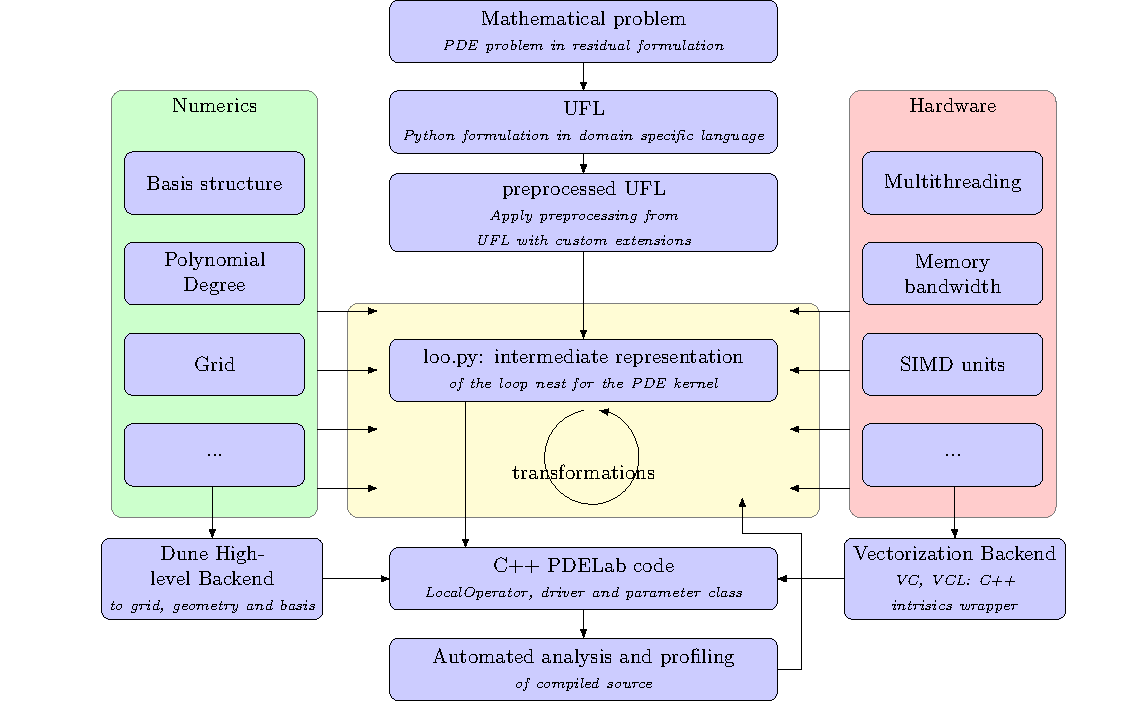
\includegraphics[width=4.5in]{figures/approach.pdf}
\end{frame}

\begin{frame}
  \lstinline{dune-codegen}, UFL, Workflow, Goal, Interface to \lstinline{dune-pdelab}
\end{frame}


\section{Writing down PDEs}

\begin{frame}
  \frametitle{Poisson}
  Discrete weak formulation: Find $u_h \in U_h$ with
  \begin{equation*}
    r_h^{Poisson}(u_h, v_h) = \int_\Omega \nabla u_h \cdot \nabla v_h \, dx
    - \int_\Omega f \, v_h \, dx = 0 \qquad \forall v_h \in V_h
  \end{equation*}

  UFL file:
  \lstinputlisting[basicstyle=\scriptsize, backgroundcolor=\color{listingbg},
]{../src/poisson.ufl}
\end{frame}

\begin{frame}[fragile]
  \frametitle{UFL: \lstinline{FiniteElement}}
  \begin{lstlisting}
V = FiniteElement(family, cell, degree)
  \end{lstlisting}
  \vfill
  \begin{itemize}
  \item family: String representing a finite element family
    \begin{itemize}
    \item \lstinline{'CG'} Continuous Lagrange finite element
    \item \lstinline{'DG'} Discontinuous Galerkin Lagrange finite element
    \end{itemize}
  \item Possible Cells:
    \begin{tabu}{ccc}
      Dimension & Simplex Cell & Cube Cell \\
      $0$ & \lstinline{vertex} & \lstinline{vertex} \\
      $1$ & \lstinline{interval} & \lstinline{interval} \\
      $2$ & \lstinline{triangle} & \lstinline{quadrilateral} \\
      $3$ & \lstinline{tetrahedron} & \lstinline{hexahedron} \\
    \end{tabu}
  \item Instead you can also write \lstinline{Cell('triangle')}
  \item \lstinline{degree}: Polynomial degree
  \end{itemize}
\end{frame}

\begin{frame}
  \frametitle{UFL: Form}
  \begin{itemize}
  \item UFL expresses forms
    \begin{align*}
      a: W_1\times\dots\times W_m\times V_1\times\dots\times V_n & \rightarrow \mathbb{R} \\
      (w_1,\dots ,w_m,v_1,\dots ,v_n) & \mapsto a(w_1,\dots ,w_m;v_1,\dots ,v_n)
    \end{align*}
  \item Linear in the arguments $v_1,\dots,v_n$
  \item Possibly nonlinear in coefficient functions $w_1,\dots,w_m$
  \item PDELab uses a residual formulation: Find $u\in U$ with
    \begin{align*}
      r(u,v) = 0 \qquad \forall v \in V
    \end{align*}
  \item $r$ is linear in $v$ but might be nonlinear in $u$
  \end{itemize}
\end{frame}

\begin{frame}[fragile]
  \frametitle{UFL: \lstinline{TrialFunction} and \lstinline{TestFunction}}

  \lstinputlisting[basicstyle=\scriptsize, backgroundcolor=\color{listingbg}, linerange={3-4}]{../src/poisson.ufl}
  \vfill
  \begin{itemize}
  \item \lstinline{TrialFunction} and \lstinline{TestFunction} represent finite element functions.
  \item Take \lstinline{FiniteElement} as argument
  \item Note: In contrast to UFL our forms need not be linear in the \lstinline{TrailFunction}
  \end{itemize}
\end{frame}

\begin{frame}
  \frametitle{UFL: Defining Expressions}
  \lstinputlisting[basicstyle=\scriptsize, backgroundcolor=\color{listingbg}, linerange={6-11}]{../src/poisson.ufl}
  \vfill
  \begin{itemize}
  \item \lstinline{SpatialCoordinate}: Global coordinate
  \item \lstinline{grad(u)}: Gradient of $u$
  \item \lstinline{inner(A,B)}: Inner product
    \begin{equation*}
      A:B = \sum_{i_0}\cdots\sum_{i_{n-1}}A_{i_0\cdots i_{n-1}}B_{i_0\cdots i_{n-1}}
    \end{equation*}
  \item \lstinline{dx}: Volume integral over cell $\int_T \cdots \, dx$
  \end{itemize}
\end{frame}

\begin{frame}
  \frametitle{UFL: \lstinline{dune-codegen} Specific}
  \lstinputlisting[basicstyle=\scriptsize, backgroundcolor=\color{listingbg}, linerange={13-15}]{../src/poisson.ufl}
  \vfill
  \begin{itemize}
  \item Main goal of \lstinline{dune-codegen} is to generate the local integration kernel
  \item For testing and solving simple problem an automated driver can be
    generated. For the correct handling of the boundary condition we need to
    add some information to the UFL file
  \item \lstinline{exact_solution}: TODO
  \item \lstinline{interpolate_expression}: TODO
  \item \lstinline{is_dirichlet}: TODO
  \end{itemize}
\end{frame}

\begin{frame}[fragile]
  \frametitle{TODO}

  UFL: triangle, FiniteElement, TrialFunction, TestFunction, SpatialCoordinate, grad, inner, dx

  dune-codegen: exact\_solution?, interpolate expression, is\_dirichlet

  TODO: VectorElement, MixedElement
\end{frame}

\begin{frame}
  \frametitle{Nonlinear Poisson}

    Strong formulation:
    \begin{align*}
      -\Delta u + q(u) & = f \qquad\text{in $\Omega\subset\mathbb{R}^d$}, \\
      u &= g \qquad\text{on $\Gamma_D\subset\partial\Omega$}, \\
      -\nabla u \cdot \mu &= j \qquad\text{on $\Gamma_N\subset\partial\Omega$}
    \end{align*}

    Weak formulation: Find $u_h \in U_h$ with
    \begin{align*}
      r_h^{NLP}(u_h, v_h) & =
      \int_\Omega \nabla u_h \cdot \nabla v_h \, dx
      + \int_\Omega q(u) \, v \, dx \\
      &\quad - \int_\Omega f \, v_h \, dx
      + \int_{\Gamma_N} j \, v \, ds
      = 0 \qquad \forall v_h \in V_h
    \end{align*}

    Parameter functions:
    \begin{align*}
      f(x) = -2d \\
      g(x) = \| x \|_2^2
    \end{align*}

    TODO: Neumann Boundary
\end{frame}

\begin{frame}
  \frametitle{UFL: Adding the Nonlinearity}
  \begin{itemize}
  \item Adjust parameter functions $f$ and $g$
  \item Define nonlinearity
  \item Add nonlinearity to residual
  \end{itemize}

  \vfill

  \lstinputlisting[basicstyle=\scriptsize,
  linerange={6-15}]{../src/nonlinear_poisson.ufl}

  TODO: Neumann Boundary
\end{frame}

\begin{frame}
  UFL: Different types of boundary
\end{frame}

\begin{frame}
  \frametitle{UFL: Using Nitsche Boundary Condition}
  TODO: Formulation

  \begin{itemize}
  \item Add Nitsche boundary implementation
  \item Remove \lstinline{is_dirichlet} part, since the boundary condition is not built into the ansatz space.
  \end{itemize}

  \vfill

  \lstinputlisting[basicstyle=\scriptsize,
  linerange={18-26}]{../src/nonlinear_poisson_nitschebc.ufl}

  TODO: Neumann Boundary
\end{frame}

\begin{frame}
  \frametitle{Something about instationary?}
\end{frame}

\begin{frame}
  \frametitle{UFL language}
  jump, avg, normal,
\end{frame}

\section{Build System Integration}

\begin{frame}[fragile]
  \frametitle{CMake: \lstinline{dune_add_generated_executable}}

  \begin{itemize}
  \item We need to generate \CC\ code and compile it
  \item Add a code generation target to your \lstinline{CMakeLists.txt}
    \inputminted[fontsize=\scriptsize]{cmake}{generated_executable.txt}
  \item \lstinline{UFLFILE}: UFL file describing the PDE
  \item \lstinline{INIFILE}: Ini file with code generation option under \lstinline{[formcompiler]} section
  \item \lstinline{TARGET}: Name of the executable
  \item \lstinline{SOURCE}: \CC\ file used for building the target. This is
    optional, if omitted a minimal driver willl be generated
  \end{itemize}
\end{frame}

\begin{frame}[fragile]
  \frametitle{CMake: \lstinline{dune_add_generated_executable}}

  \begin{itemize}
  \item Automated driver generation is mainly developed for software tests
  \item For complicated applications handwritten drivers will be
    necessary. This requires control over the file- and classname of the
    generated local operator.
  \item Can be done in the ini file \vspace{0.3cm}
    \inputminted[fontsize=\scriptsize]{ini}{classname_filename.ini}
  \end{itemize}
\end{frame}

\begin{frame}[fragile]
  \frametitle{Options?}

  Global Options:

  \begin{lstlisting}
  explicit_time_stepping
  exact_solution_expression
  compare_l2errorsquared
  \end{lstlisting}

  Form Options:

  \begin{lstlisting}
  filename
  classname
  ? numerical_jacobian
  quadrature_order
  geometry_mixins
  ? enable_volume
  ? enable_skeleton
  ? enable_boundary
  \end{lstlisting}
\end{frame}

\begin{frame}[fragile]
  \frametitle{CMake: \lstinline{dune_add_generated_executable}}

  TODO: Maybe add an example where we do not generate a driver to have a meaningful example.
  \vfill
  \lstinline{CMakeLists.txt}
  \inputminted[fontsize=\scriptsize, firstline=1, lastline=4]{cmake}{../src/CMakeLists.txt}
  \vfill
  \lstinline{poison.ini}
  \inputminted[fontsize=\scriptsize]{ini}{../src/poisson.ini}
\end{frame}

\begin{frame}
  TODO: Slide for the inspire course how to navigate the exercise
\end{frame}

\end{document}
